\razdelek{Celoštevilsko linearno programiranje}

\begin{naloga}{?}{Vaje OR 16.3.2016}
\begin{vprasanje}[proj]
Občina Ljubljana želi projekte iz množice
$\p = \{p_1, p_2, \dots, p_n\}$,
pri čemer ima na voljo $M$ evrov kapitala.
V želji po razvoju regije želijo,
da se v sklopu sponzoriranih projektov ustvari vsaj $N$ delovnih mest.
Projekt $p_i$ ($1 \le i \le n)$ potrebuje $d_i$ evrov finančne pomoči
in zaposli $a_i$ ljudi.
Na občini so ocenili,
da ima projekt $p_i$ ob uspešnem dokončanju donos $c_i$ evrov.
Katere projekte naj sponzorira, da bo donos čim večji?
Na smiseln način modeliraj opisani problem z linearnim programom.
\end{vprasanje}

\begin{odgovor}
Za vsak projekt $p_i \in \p$ bomo uvedli spremenljivko $x_i$,
katere vrednost interpretiramo kot
$$
x_i = \begin{cases}
1, & \text{če naj občina sponzorira projekt $p_i$, in} \\
0  & \text{sicer.}
\end{cases}
$$
Zapišimo celoštevilski linearni program.
\begin{alignat*}{2}
\max \ \sum_{i=1}^n c_i x_i && \text{p.p.} \\
\forall i \in \{1, \dots, n\}: &\ & 0 \le x_i &\le 1, \quad x_i \in \Z \\
&& \sum_{i=1}^n d_i x_i &\le M \\
&& \sum_{i=1}^n a_i x_i &\ge N
\end{alignat*}
\end{odgovor}
\end{naloga}


\begin{naloga}{?}{Vaje OR 16.3.2016}
\begin{vprasanje}
Obravnavajmo posplošen scenarij iz naloge~\nal{proj}.
\begin{enumerate}[(a)]
\item Denimo, da so projekti lahko med seboj odvisni.
Imejmo množico $V \subseteq \p^2$, ki določa,
da za vsak par projektov $(p_i, p_j) \in V$ velja,
da lahko projekt $p_i$ sponzoriramo le,
če sponzoriramo tudi projekt $p_j$.

\item Nekateri izmed projektov so lahko v konfliktu.
Naj bo $S \subseteq 2^\p$ družina množic, ki določa,
da so za vsako množico $H \in S$ projekti iz $H$ med seboj v konfliktu
(tj., hkrati lahko sponzoriramo le enega izmed njih.)
\end{enumerate}
Opiši, kako bi modelirali opisane omejitve.
\end{vprasanje}

\begin{odgovor}
Celoštevilskemu linearnemu programu iz rešitve naloge~\res{proj}
bomo dodali nove omejitve.
\begin{enumerate}[(a)]
\item $\displaystyle \forall (p_i, p_j) \in V : x_i \le x_j$
\item $\displaystyle \forall H \in S : \sum_{p_i \in H} x_i \le 1$
\end{enumerate}
\end{odgovor}
\end{naloga}


\begin{naloga}[problem prevoza in skladiščenja dobrin]{?}{Vaje OR 16.3.2016}
\begin{vprasanje}
V Evropski uniji je na voljo $n$ skladišč,
pri čemer znašajo stroški najema $i$-tega skladišča $f_i$
(ne glede na zasedenost),
vsako skladišče pa lahko hrani enoto dobrine.
Imamo $m$ strank, ki jim dostavljamo dobrine,
pri čemer $c_{ij}$ ($1 \le i \le n$, $1 \le j \le m$)
predstavlja strošek dostave dobrine stranki $j$ iz skladišča $i$.
Predpostavimo tudi, da ima vsaka stranka določeno potrebo $d_j$,
ki ponazarja število enot dobrine, ki jo potrebuje.
V katerih skladiščih naj hranimo dobrine,
da bodo skupni stroški najema in dostave čim manjši?
Na smiseln način modeliraj opisani problem z linearnim programom.
\end{vprasanje}

\begin{odgovor}
Za vsako skladišče, ki ga uporabimo,
želimo vedeti, kateri stranki bomo dostavili dobrino.
Za $i$-to skladišče ($1 \le i \le n$) in $j$-to stranko ($1 \le j \le m$)
bomo uvedli spremenljivko $x_{ij}$,
katere vrednost interpretiramo kot
$$
x_{ij} = \begin{cases}
1, & \text{če bomo iz $i$-tega skladišča dostavili $j$-ti stranki, in} \\
0  & \text{sicer.}
\end{cases}
$$
Zapišimo celoštevilski linearni program.
\begin{alignat*}{2}
\min \ \sum_{i=1}^n \sum_{j=1}^m (f_i + c_{ij}) x_{ij} && \text{p.p.} \\
\forall i \in \{1, \dots, n\} \ \forall j \in \{1, \dots, m\}: &\ &
0 \le x_{ij} &\le 1, \quad x_{ij} \in \Z
\opis{Vsako skladišče uporabimo največ enkrat}
\forall i \in \{1, \dots, n\}: &\ & \sum_{j=1}^m x_{ij} &\le 1
\opis{Zadostimo potrebe vsake stranke}
\forall j \in \{1, \dots, m\}: &\ & \sum_{i=1}^n x_{ij} &\ge d_j
\end{alignat*}
\end{odgovor}
\end{naloga}


\begin{naloga}[problem kombinatorične dražbe]%
{Sergio Cabello}{Vaje OR 5.3.2018}
\begin{vprasanje}
Dražitelj ponuja predmete iz množice $A$
in prejme ponudbe $\{(B_i, c_i)\}_{i=1}^k$,
pri čemer je $c_i$ cena,
ki jo udeleženec dražbe ponudi za predmete v množici $B_i \subseteq A$.
Katere ponudbe naj dražitelj sprejme,
da maksimizira dobiček,
če lahko vsak predmet proda največ enkrat?
Modeliraj opisani problem z linearnim programom.
\end{vprasanje}

\begin{odgovor}
Za $i$-to ponudbo ($1 \le i \le k$) bomo uvedli spremenljivko $x_i$,
katere vrednost interpretiramo kot
$$
x_i = \begin{cases}
1, & \text{če naj dražitelj sprejme $i$-to ponudbo, in} \\
0  & \text{sicer.}
\end{cases}
$$
Zapišimo celoštevilski linearni program.
\begin{alignat*}{2}
\max \ \sum_{i=1}^n c_i x_i && \text{p.p.} \\
\forall i \in \{1, \dots, k\}: &\ & 0 \le x_i &\le 1, \quad x_i \in \Z \\
\forall p \in A: &\ & \sum_{\substack{i=1 \\ p \in B_i}}^k x_i &\le 1
\end{alignat*}
\end{odgovor}
\end{naloga}


\begin{naloga}{?}{Vaje OR 16.3.2016}
\begin{vprasanje}
Definiraj problem dominacijske množice v grafu
in zapiši celoštevilski linearni program,
ki rešuje opisani problem.
\end{vprasanje}

\begin{odgovor}
Naj bo $G = (V, E)$ neusmerjen graf.
Množica $D \subseteq V$ {\em dominira} graf $G$
če je vsako vozlišče iz $V$ bodisi v $D$, bodisi ima soseda v $D$.
Pri problemu dominacijske množice iščemo najmanjšo množico $D_{\min}$,
ki dominira graf $G$.

Za vsako vozlišče $v \in V$ bomo uvedli spremenljivko $x_v$,
katere vrednost interpretiramo kot
$$
x_v = \begin{cases}
1, & \text{vozlišče $v$ je v množici $D_{\min}$, in} \\
0  & \text{sicer.}
\end{cases}
$$
Zapišimo celoštevilski linearni program.
\begin{alignat*}{2}
&& \min \ \sum_{v \in V} x_v &\quad \text{p.p.} \\
\forall v \in V: &\ & 0 \le x_v &\le 1, \quad x_v \in \Z \\
\forall v \in V: &\ & x_v + \sum_{uv \in E} x_u &\ge 1
\end{alignat*}
\end{odgovor}
\end{naloga}


\begin{naloga}{Janoš Vidali}{Vaje OR 12.10.2016}
\begin{vprasanje}
Napiši linearni program,
ki modelira iskanje največjega prirejanja v dvodelnem grafu.
\end{vprasanje}

\begin{odgovor}
Naj bo $G = (V, E)$ dvodelen graf.
Lahko torej zapišemo $V = A \cup B$ tako,
da sta množici $A$ in $B$ disjunktni
ter za vsako povezavo $uv \in E$ velja $u \in A$, $v \in B$.
Množica $M \subset E$ je {\em prirejanje},
če nobeni dve povezavi iz $M$ nimata skupnega krajišča.
Iščemo največje prirejanje $M_{\max}$.

Za vsako povezavo $uv \in E$ bomo uvedli spremenljivko $x_{uv}$,
katere vrednost interpretiramo kot
$$
x_{uv} = \begin{cases}
1, & \text{povezava $uv$ je v množici $M_{\max}$, in} \\
0  & \text{sicer.}
\end{cases}
$$
Zapišimo celoštevilski linearni program.
\begin{alignat*}{2}
\max &\ & \sum_{uv \in E} x_{uv} &\quad \text{p.p.} \\
\forall uv \in E: &\ & 0 \le x_{uv} &\le 1, \quad x_{uv} \in \Z \\
\forall u \in A: &\ & \sum_{uv \in E} x_{uv} &\le 1 \\
\forall v \in B: &\ & \sum_{uv \in E} x_{uv} &\le 1
\end{alignat*}
\end{odgovor}
\end{naloga}


\begin{naloga}{?}{Vaje OR 16.3.2016}
\begin{vprasanje}
Napiši linearni program,
ki modelira iskanje najkrajše poti
med danima vozliščema $u$ in $v$ v usmerjenem grafu $G$.
\end{vprasanje}

\begin{odgovor}
Naj bo $G = (V, E)$ usmerjen graf in $u, v \in V$ njegovi vozlišči.
Poiskati želimo najkrajšo pot $P_{uv}$ od vozlišča $u$ do vozlišča $v$.

Za vsako povezavo $uv \in E$ bomo uvedli spremenljivko $x_{uv}$,
katere vrednost interpretiramo kot
$$
x_{uv} = \begin{cases}
1, & \text{povezava $uv$ je v poti $P_{uv}$, in} \\
0  & \text{sicer.}
\end{cases}
$$
Zapišimo celoštevilski linearni program.
\begin{alignat*}{2}
&& \min \ \sum_{uv \in E} x_{uv} &\quad \text{p.p.} \\
\forall uv \in E: &\ & 0 \le x_{uv} &\le 1, \quad x_{uv} \in \Z
\opis{Iz vozlišča $u$ izstopimo enkrat več kakor vstopimo}
&& \sum_{yu \in E} x_{yu} - \sum_{uz \in E} x_{uz} &= -1
\opis{V vozlišče $v$ vstopimo enkrat več kakor izstopimo}
&& \sum_{yv \in E} x_{yv} - \sum_{vz \in E} x_{vz} &= 1
\opis{V ostala vozlišča vstopimo natanko tolikokrat kakor vstopimo}
\forall w \in V \setminus \{u, v\}: &\ &
\sum_{yw \in E} x_{yw} - \sum_{wz \in E} x_{wz} &= 0
\end{alignat*}
Zgornje omejitve sicer dovolijo, da posamezno vozlišče obiščemo večkrat,
a se je mogoče teh zank znebiti,
pri čemer se vrednost ciljne funkcije zmanjša.
Tako bo optimalna rešitev zagotovo pot od vozlišča $u$ do vozlišča $v$.
\end{odgovor}
\end{naloga}


\begin{naloga}{?}{Izpit OR 28.8.2013}
\begin{vprasanje}
Kukavica bo izlegla $16$ jajc in jih podtaknila v $12$ gnezd,
ki pripadajo dvema taščicama, štirim vrtnim penicam, trem travniškim cipam,
dvema belima pastiricama in eni sovi.
V vsako gnezdo lahko izleže največ tri jajca,
pri čemer je verjetnost, da mladiči v gnezdu $i$ preživijo,
enaka $p_{ij}$, kjer je $j$ število podtaknjenih jajc v gnezdu $i$
(preživijo bodisi vsi ali noben mladič v posameznem gnezdu).
Pri vsaki od petih vrst ptic želi izleči vsaj eno jajce,
pri taščicah pa želi izleči strogo več jajc kot pri belih pastiricah.
Poleg tega pri drugi beli pastirici ne bo odložila jajca,
če bo pri prvi taščici odložila dve jajci ali več.
Kukavica želi maksimizirati pričakovano število preživelih mladičev.

Zapiši problem kot celoštevilski linearni program.
\end{vprasanje}

\begin{odgovor}
Oštevilčimo gnezda s števili od $1$ do $12$:
gnezdi taščic naj imata števili $1$ in $2$,
gnezda vrtnih penic naj imajo števila $3$ in $4$, $5$ in $6$,
gnezda travniških cip naj imajo števila $7$ in $8$, in $9$,
gnezdi belih pastiric naj imata števili $10$ in $11$,
sovino gnezdo pa naj ima število $12$.
Za $i$-to gnezdo ($1 \le i \le 12$) in $j \in \{1, 2, 3\}$
bomo uvedli spremenljivko $x_{ij}$,
katere vrednost interpretiramo kot
$$
x_{ij} = \begin{cases}
1, & \text{če naj kukavica v $i$-to gnezdo izleže natanko $j$ jajc, in} \\
0  & \text{sicer.}
\end{cases}
$$
Naj bo $V = \{\{1, 2\}, \{3, 4, 5, 6\}, \{7, 8, 9\}, \{10, 11\}, \{12\}\}$
particija indeksov gnezd glede na vrsto ptice.
Zapišimo celoštevilski linearni program.
\begin{align*}
\max \ \sum_{i=1}^{12} j \ p_{ij} \ x_{ij} &\quad \text{p.p.} \\
\forall i \in \{1, \dots, 12\}: \ \sum_{j=1}^3 x_{ij} &\le 1
\opis{Skupaj izleže $16$ jajc}
\sum_{i=1}^{12} \sum_{j=1}^3 j \ x_{ij} &= 16
\opis{K vsaki vrsti ptice izleže vsaj eno jajce}
\forall S \in V: \ \sum_{i \in S} \sum_{j=1}^3 x_{ij} &\ge 1
\opis{Pri taščicah izleže strogo več jajc kot pri belih pastiricah}
\sum_{i=1}^2 \sum_{j=1}^3 j \ x_{ij} - \sum_{i=10}^{11} \sum_{j=1}^3 j \ x_{ij} &\ge 1
\opis{Pri drugi beli pastirici ne bo odložila jajca,
če bo pri prvi taščici odložila dve jajci ali več}
\sum_{j=2}^3 x_{1j} + \sum_{j=1}^3 x_{11,j} &\le 1
\end{align*}
\end{odgovor}
\end{naloga}


\begin{naloga}{?}{Kolokvij OR 31.5.2012}
\begin{vprasanje}[vinar]
Vinar Janez je pridelal $2000$ litrov rumenega muškata,
$10000$ litrov laškega rizlinga in $5000$ litrov renskega rizlinga.
Njegovi kupci so bara Kocka in Luka ter župnišče Sv.~Martin in občina Duplek.
Vsak od njih je pripravljen kupiti največ določeno količino vina
po fiksni ceni, ne glede na sorto:

\begin{center}
\begin{tabular}{r|cccc}
kupec & Kocka & Luka & župnišče & občina \\ \hline
cena za liter & $1.0$ & $1.1$ & $1.5$ & $1.8$ \\
največja količina v litrih & $15000$ & $5000$ & $500$ & $1000$ \\
\end{tabular}
\end{center}

Janez se je odločil, da bo vsako sorto prodal največ enemu kupcu,
in sicer v maksimalni količini
(če kupec ne kupi vsega vina iste sorte, ga Janez ohrani zase).
Župan pravi, da občina drugega vina kot renskega rizlinga ne bo kupila.
Bar Luka želi rumeni muškat, če bar Kocka dobi laški rizling.
Pri Kocki so se dogovorili, da če občina in župnišče ne kupijo nič,
tudi oni ne bodo kupili ničesar.
Janezova žena pa vztraja,
da če kupec $A$ kupi sorto $s_A$ in kupec $B$ kupi sorto $s_B$,
potem naj sorta $s_C$ ostane doma ali jo kupi kupec $C$ (za neke $A, B, C$).
Kako naj Janez proda vino, da bo čim več zaslužil?

Zapiši problem kot celoštevilski linearni program.
\end{vprasanje}

\begin{odgovor}
Za vsako sorto $i \in I = \{RM, LR, RR\}$
(rumeni muškat, laški rizling, renski rizling)
in kupca $j \in J = \{K, L, Z, O\}$
(bar Kocka, bar Luka, župnišče Sv. Martin, občina Duplek)
bomo uvedli spremenljivko $x_{ij}$,
katere vrednost interpretiramo kot
$$
x_{ij} = \begin{cases}
1, & \text{če naj Janez proda sorto $i$ kupcu $j$, in} \\
0  & \text{sicer.}
\end{cases}
$$
Zapišimo celoštevilski linearni program.
\begin{gather*}
\begin{alignedat}{4}
\max &\ 2000 x_{RM, K} &&+ 2200 x_{RM, L} &&+ 750 x_{RM, Z} &&+ 1800 x_{RM, O} \\
{}+ &\ 10000 x_{LR, K} &&+ 5500 x_{LR, L} &&+ 750 x_{LR, Z} &&+ 1800 x_{LR, O} \\
{}+ &\ 5000 x_{RR, K}  &&+ 5500 x_{RR, L} &&+ 750 x_{RR, Z} &&+ 1800 x_{RR, O}
\quad \text{p.p.}
\end{alignedat} \\
\begin{aligned}
\forall i \in I \ \forall j \in J: \ 0 \le x_{ij} &\le 1, \quad x_{ij} \in \Z
\opis{Vsako sorto proda največ enemu kupcu}
\forall i \in I: \sum_{j \in J} x_{ij} &\le 1
\opis{Vsak kupec dobi največ eno sorto}
\forall j \in J: \sum_{i \in I} x_{ij} &\le 1
\opis{Občina ne bo kupila rumenega muškata ali laškega rizlinga}
x_{RM, O} + x_{LR, O} &= 0
\opis{Če Kocka dobi laški rizling, potem Luka dobi rumeni muškat}
x_{LR, K} &\le x_{RM, L}
\opis{Če občina in župnišče ne kupita ničesar, tudi Kocka ne kupi ničesar}
\sum_{i \in I} (x_{i, O} + x_{i, Z} - x_{i, K}) &\ge 0
\opis{Ženin pogoj}
x_{s_A, A} + x_{s_B, B} + \sum_{j \in J \setminus \{C\}} x_{s_C, j} &\le 2
\end{aligned}
\end{gather*}
\end{odgovor}
\end{naloga}

\begin{naloga}{?}{Vaje OR 16.3.2016}
\begin{vprasanje}
Napiši linearni program,
ki poišče razdalje od danega vozlišča $u$ v grafu $G$.
\end{vprasanje}

\begin{odgovor}
Graf $G = (V, E)$ smatramo kot usmerjen graf
(če je dani graf ne\-usme\-rjen,
vsako povezavo nadomestimo s parom nasprotno usmerjenih povezav).
Naj bo $n = |V|$ število vozlišč grafa $G$.
Rešitev celoštevilskega linearnega programa
predstavlja usmerjeno drevo najkrajših poti s korenom v vozlišču $u$.

Za vsako povezavo $vw \in E$ bomo uvedli spremenljivko $x_{vw}$,
katere vrednost interpretiramo kot
$$
x_{vw} = \begin{cases}
1, & \text{povezava $vw$ je v drevesu najkrajših poti, in} \\
0  & \text{sicer.}
\end{cases}
$$
Poleg tega bomo za vsako vozlišče $v \in V$
uvedli še spremenljivko $y_v$,
ki nam pove razdaljo od vozlišča $u$ do vozlišča $v$.
Minimizirati želimo vse vrednosti $y_v$, zato bomo minimizirali njihovo vsoto.

Zapišimo celoštevilski linearni program.
\begin{alignat*}{2}
&& \min &\ \sum_{v \in V} y_v \quad \text{p.p.} \\
\forall vw \in E: &\ & 0 \le x_{vw} &\le 1, \quad x_{vw} \in \Z
\opis{Vozlišče $u$ nima vstopne povezave v drevesu}
&& \sum_{vu \in E} x_{vu} &= 0
\opis{Ostala vozlišča imajo natanko eno vstopno povezavo v drevesu}
\forall vw \in E, & \ v \ne u: \ & \sum_{vw \in E} x_{vw} &= 1
\opis{Vozlišče $u$ je na razdalji $0$ od sebe}
&& y_u &= 0
\opis{Če je povezava $vw$ v drevesu,
je razdalja do $w$ vsaj za $1$ večja od razdalje do $v$,
sicer pa je razlika največ $n-1$}
\forall vw \in E: &\ & y_v + n x_{vw} &\le y_w + n - 1
\opis{V drevesu je natanko $n-1$ povezav}
&& \sum_{vw \in e} x_{vw} &= n-1
\end{alignat*}
\end{odgovor}
\end{naloga}


\begin{naloga}{?}{Vaje OR 16.3.2016}
\begin{vprasanje}
Napiši linearni program,
ki modelira določanje kromatičnega števila grafa.
\end{vprasanje}

\begin{odgovor}
{\em Pravilno barvanje} (neusmerjenega) grafa $G = (V, E)$
je taka dodelitev barv vozliščem grafa $G$,
da imata krajišči vsake povezave različno barvo.
{\em Kromatično število} grafa $G$ je najmanjše število barv,
ki jih potrebujemo za pravilno barvanje grafa $G$.

Naj bo $n = |V|$ število vozlišč grafa $G$
-- to je tudi največje število barv, ki jih lahko uporabimo.
Za vsako vozlišče $v \in V$ in vsako barvo $i$ ($1 \le i \le n$)
bomo uvedli spremenljivko $x_{vi}$,
katere vrednost interpretiramo kot
$$
x_{vi} = \begin{cases}
1, & \text{vozlišče $v$ pobarvamo z barvo $i$, in} \\
0  & \text{sicer.}
\end{cases}
$$
Poleg tega bomo uvedli še spremenljivko $t$, ki šteje uporabljene barve.

Zapišimo celoštevilski linearni program.
\begin{alignat*}{2}
&& \min &\ t \quad \text{p.p.} \\
\forall v \in V \ \forall i \in \{1, \dots, n\}: &\ &
0 \le x_{vi} &\le 1, \quad x_{vi} \in \Z
\opis{Vsako vozlišče je natanko ene barve}
\forall v \in V: &\ & \sum_{i=1}^n x_{vi} &= 1
\opis{Krajišči povezav sta različnih barv}
\forall uv \in E \ \forall i \in \{1, \dots, n\}: &\ &
x_{ui} + x_{vi} &\le 1
\opis{Omejimo $t$ z indeksi uporabljenih barv}
\forall uv \in E \ \forall i \in \{1, \dots, n\}: &\ &
i x_{vi} &\le t
\end{alignat*}
\end{odgovor}
\end{naloga}


\begin{naloga}[problem trgovskega potnika]{?}{Vaje OR 16.3.2016}
\begin{vprasanje}[tsp]
Danih je $n$ mest na zemljevidu.
Strošek potovanja iz mesta $i$ v mesto $j$ je $c_{ij}$ ($1 \le i, j \le n$).
Trgovski potnik želi obiskati vseh $n$ mest,
pri tem pa minimizirati strošek potovanja.
Na smiseln način modeliraj opisani problem z linearnim programom.
\end{vprasanje}

\begin{odgovor}
Pot bomo opisali z množico povezav v polnem grafu z $n$ vozlišči (mesti),
ki tvorijo cikel.
Za vsak par mest $(i, j)$ ($1 \le i, j \le n$)
bomo uvedli spremenljivko $x_{ij}$,
katere vrednost interpretiramo kot
$$
x_{ij} = \begin{cases}
1, & \text{iz $i$-tega mesta odpotujemo v $j$-to mesto} \\
0  & \text{sicer.}
\end{cases}
$$
Poskrbeti bomo morali še,
da bo naša rešitev res sestavljena iz enega samega cikla.
V ta namen bomo za $i$-to mesto ($1 \le i \le n$) uvedli spremenljivko $y_i$,
ki pove, katero po vrsti smo to mesto obiskali.
Ker je rešitev cikel, si lahko poljubno izberemo,
katero je prvo obiskano mesto (npr.~mesto z indeksom $1$).

Zapišimo celoštevilski linearni program.
\begin{alignat*}{2}
\min \ \sum_{i=1}^n \sum_{j=1}^n x_{ij} c_{ij} && \text{p.p.}\\
\forall i, j \in \{1, \dots, n\}: &\ &
0 \le x_{ij} &\le 1, \quad x_{ij} \in \Z
\opis{V vsako mesto prispemo natanko enkrat}
\forall j \in \{1, \dots, n\}: &\ & \sum_{i=1}^n x_{ij} &= 1
\opis{Vsako mesto zapustimo natanko enkrat}
\forall i \in \{1, \dots, n\}: &\ & \sum_{i=1}^n x_{ij} &= 1
\opis{Če iz mesta $i$ potujemo v mesto $j > 1$, mu to sledi v vrstnem redu}
\forall i  \in \{1, \dots, n\} \ \forall j \in \{2, \dots, n\}: &\ &
y_i + n x_{ij} &\le y_j + n - 1
\end{alignat*}
\end{odgovor}
Zadnji pogoj poskrbi, da rešitev nima cikla brez mesta z indeksom $1$.
Skupaj s pogojema, da vsako mesto obiščemo in zapustimo natanko enkrat,
si tako zagotovimo, da bo rešitev obsegala natanko en cikel.
Vrednost spremenljivk $y_i$ ($1 \le i \le n$) ni omejena
-- zadnji pogoj poskrbi le, da je največja razlika med njimi enaka $n-1$.
\end{naloga}


\begin{naloga}{?}{Vaje OR 23.3.2016}
\begin{vprasanje}
S celoštevilskim linearnim programom
modeliraj problem iskanja minimalnega vpetega drevesa v grafu.
\end{vprasanje}

\begin{odgovor}
Denimo, da imamo usmerjen graf $G = (V, E)$,
kjer ima vsaka povezava $uv \in E$ svojo ceno $c_{uv}$
(če je dani graf ne\-usme\-rjen,
vsako povezavo nadomestimo s parom nasprotno usmerjenih povezav z isto ceno).
Minimalno vpeto drevo je drevo $T = (V, E')$ z $E' \subseteq E$,
za katerega je vsota cen povezav iz $E'$ najmanjša.

Naj bo $n = |V|$ število vozlišč grafa $G$.
Za vsako povezavo $uv \in E$ bomo uvedli spremenljivko $x_{uv}$,
katere vrednost interpretiramo kot
$$
x_{uv} = \begin{cases}
1, & \text{povezava $uv$ je v množici $E'$, in} \\
0  & \text{sicer.}
\end{cases}
$$
Poskrbeti moramo še, da bo naša rešitev res drevo.
Izberimo si vozlišče $r \in V$ kot koren drevesa
in za vsako vozlišče $v \in V$ uvedimo še spremenljivko $y_v$,
ki se povečuje z globino vozlišča v drevesu.

Zapišimo celoštevilski linearni program.
\begin{alignat*}{2}
\min &\ & \sum_{uv \in E} x_{uv} c_{uv} &\quad \text{p.p.} \\
\forall uv \in E: &\ & 0 \le x_{uv} &\le 1, \quad x_{uv} \in \Z
\opis{V vozlišče $r$ ne vstopi nobena povezava v drevesu}
&& \sum_{ur \in E} x_{ur} &= 0
\opis{V ostala vozlišča vstopi natanko ena povezava}
\forall u \in V \setminus \{r\}: &\ & \sum_{uv \in E} x_{uv} &= 1
\opis{Vrednost $y_v$ ($v \in V$) se povečeje po povezavah iz drevesa}
\forall uv \in E: &\ & y_u + n x_{uv} &\le y_v + n - 1
\end{alignat*}
Zadnji pogoj poskrbi,
da so vsa vozlišča v drevesu in ne v nepovezanem ciklu.
Podobno kot pri nalogi~\res{tsp}
vrednost spremenljivk $y_v$ ($v \in V$) ni omejena
-- pogoj poskrbi le, da je največja razlika med njimi največ $n-1$.
\end{odgovor}
\end{naloga}


\begin{naloga}{Janoš Vidali}{Izpit OR 15.12.2016}
\begin{vprasanje}
Na oddelku za matematiko je zaposlenih $n$ asistentov,
ki jim moramo dodeliti vaje pri $m$ predmetih.
Za asistenta $i$ ($1 \le i \le n$) naj bosta $a_i$ in $b_i$
najmanjše in največje število ur, ki jih lahko izvaja,
ter $N_i \subseteq \{1, 2, \dots, m\}$ množica predmetov,
ki jih ne želi izvajati.
Za predmet $j$ ($1 \le j \le m$)
naj bo $c_j$ število skupin za vaje pri predmetu,
ter $u_j$ število ur vaj na skupino.
Poleg tega vemo, da sta asistenta $p$ in $q$ skregana,
zato pri nobenem predmetu ne smeta oba izvajati vaj.

Predmete želimo asistentom dodeliti tako,
da bomo ob upoštevanju njihovih želja
minimizirali največje število različnih predmetov,
ki smo jih dodelili posamezenmu asistentu.

Zapiši celoštevilski linearni program, ki modelira zgoraj opisani problem.
\namig{napiši program s spremenljivko $t$, ki je dopusten natanko tedaj,
ko vsak asistent dobi največ $t$ različnih predmetov,
in potem minimimiziraj $t$.}
\end{vprasanje}

\begin{odgovor}
Za $i$-tega asistenta ($1 \le i \le n$)
in $j$-ti predmet ($1 \le j \le m$)
bomo uvedli spremenljivki $x_{ij}$ in $y_{ij}$,
kjer je $x_{ij}$ število skupin,
ki jih $i$-temu asistentu dodelimo pri $j$-tem predmetu,
vrednost $y_{ij}$ pa interpretiramo kot
$$
y_{ij} = \begin{cases}
1, & \text{$i$-ti asistentu bo izvajal vaje pri $j$-tem predmetu, in} \\
0  & \text{sicer.}
\end{cases}
$$
Poleg tega bomo uvedli še spremenljivko $t$,
s katero omejimo največje število različnih predmetov
pri posameznem asistentu.

Zapišimo celoštevilski linearni program.
\begin{alignat*}{2}
&& \min &\ t \quad \text{p.p.} \\
\forall i \in \{1, \dots, n\} \ \forall j \in \{1, \dots, m\}: &\ &
x_{ij} &\ge 0, \quad x_{ij} \in \Z \\
\forall i \in \{1, \dots, n\} \ \forall j \in \{1, \dots, m\}: &\ &
0 \le y_{ij} &\le 1, \quad y_{ij} \in \Z
\opis{$x_{ij} = 0$ natanko tedaj, ko $y_{ij} = 0$}
\forall i \in \{1, \dots, n\} \ \forall j \in \{1, \dots, m\}: &\ &
y_{ij} \le x_{ij} &\le c_j y_{ij}
\opis{Omejimo število ur za vsakega asistenta}
\forall i \in \{1, \dots, n\}: &\ & a_i \le \sum_{j=1}^m u_j x_{ij} &\le b_i
\opis{Neželenih predmetov ne dodelimo}
\forall i \in \{1, \dots, n\}: &\ & \sum_{j \in N_i} y_{ij} &= 0
\opis{Za vsak predmet dodelimo potrebno število skupin}
\forall j \in \{1, \dots, m\}: &\ & \sum_{i=1}^n x_{ij} &= c_j
\opis{Nobenega predmeta ne dodelimo asistentoma $p$ in $q$}
\forall j \in \{1, \dots, m\}: &\ & y_{pj} + y_{qj} &\le 1
\opis{Število različnih predmetov na asistenta omejimo s $t$}
\forall i \in \{1, \dots, n\}: &\ & \sum_{j=1}^n y_{ij} &\le t
\end{alignat*}
\end{odgovor}
\end{naloga}


\begin{naloga}{Janoš Vidali}{Izpit OR 31.1.2017}
\begin{vprasanje}
Imamo $m$ opravil, ki jih želimo razporediti med $n$ strojev.
Vsak stroj lahko hkrati opravlja le eno opravilo,
vsa opravila pa trajajo eno časovno enoto, neodvisno od stroja.
Če stroj $i$ ($1 \le i \le n$) uporabimo za vsaj eno opravilo,
plačamo ceno $c_i$
(cena ostane enaka, če na istem stroju naredimo več opravil).
Skupni stroški ne smejo preseči količine $C$.
Dani sta še množici parov $P$ in $S$,
pri čemer $(j, k) \in P$ pomeni,
da mora biti opravilo $j$ dokončano pred začetkom opravila $k$,
$(j, k) \in S$ pa pomeni, da se opravili $j$ in $k$ ne smeta izvajati hkrati.
Imamo še dodaten pogoj, ki zahteva,
da je lahko v posamezni časovni enoti lahko aktivnih največ $A$ strojev.
Minimizirati želimo čas dokončanja zadnjega stroja.

Zapiši celoštevilski linearni program, ki modelira zgoraj opisani problem.
\end{vprasanje}
\begin{odgovor}
\end{odgovor}
\end{naloga}


\begin{naloga}[problem polnjenja košev]{Sergio Cabello}{Izpit OR 15.3.2017}
\begin{vprasanje}
Imamo neskončno košev $B_1, B_2, \dots$,
od katerih ima vsak velikost $V > 0$,
in $n$ predmetov pozitivnih velikosti $s_1, s_2, \dots, s_n$,
od katerih je vsaka največ $V$.
Predmete želimo postaviti v koše tako, da porabimo čim manj košev,
pri čemer noben koš ne vsebuje predmetov skupne velikosti več kot $V$.
Na primer, če $V = 10$ ter $s_1 = 4$, $s_2 = 5$ in $s_3 = 7$,
lahko to storimo z dvema košema, medtem ko z enim samim košem to ni mogoče.

\begin{enumerate}[(a)]
\item Zapiši celoštevilski linearni program, ki modelira zgornji problem.

\item Denimo, da imamo seznam $L$ s pari predmetov,
ki jih ne smemo postaviti v isti koš.
Če imamo na primer $L = \{(1, 2), (3, 4), (1, 4)\}$,
potem predmetov $1$ in $2$ ne moremo postaviti skupaj,
prav tako ne predmetov $3$ in $4$ oziroma $1$ in $4$.

Dopolni zgornji celoštevilski linearni program tako,
da bo vključeval te ome\-jit\-ve.
\end{enumerate}
\end{vprasanje}
\begin{odgovor}
\end{odgovor}
\end{naloga}


\begin{naloga}{Janoš Vidali}{Izpit OR 10.7.2017}
\begin{vprasanje}
Za hitrejše nalaganje posnetkov na YouTubu se uporabljajo krajevni strežniki,
do katerih lahko uporabniki na določeni lokaciji hitreje dostopajo
kakor do glavnega strežnika, ki vsebuje vse posnetke.
Vendar pa imajo krajevni strežniki omejen prostor,
zato je potrebno ugotoviti,
kateri posnetki naj se naložijo na katere krajevne strežnike.

Denimo, da imamo poleg glavnega strežnika še $k$ krajevnih strežnikov,
$m$ internetnih po\-nud\-ni\-kov in $n$ posnetkov.
Naj bo $c_h$ ($1 \le h \le k$) prostor v megabajtih,
ki je na voljo na krajevnem strežniku $h$.
Z indeksom $0$ označimo glavni strežnik
-- lahko torej predpostavljaš $c_0 = \infty$.
Nadalje naj bo $s_j$ ($1 \le j \le n$) velikost posnetka $j$,
prav tako v megabajtih,
$\ell_{hi}$ ($0 \le h \le k$, $1 \le i \le m$)
latenca (zakasnitev pri prenosu v milisekundah)
ponudnika $i$ do strežnika $h$,
in $r_{ij}$ ($1 \le i \le m$, $1 \le j \le n$)
število zahtevkov za posnetek $j$, ki jih pričakujejo od ponudnika $i$.
Vsi parametri so cela števila.

Pri vsakem zahtevku bo posnetek poslan iz strežnika z najmanjšo latenco,
ki vsebuje želeni posnetek.
Lahko predpostavljaš,
da ima za vsakega ponudnika glavni strežnik največjo latenco
(torej $\ell_{0i} \ge \ell_{hi}$ za vsaka $1 \le h \le k$, $1 \le i \le m$).
Določiti želimo, katere posnetke naj naložimo na posamezen krajevni strežnik,
da minimiziramo vsoto pričakovanih latenc pri vseh zahtevkih.
Posamezen posnetek lahko seveda naložimo tudi na več krajevnih strežnikov,
ali pa na nobenega (v tem primeru bo poslan iz glavnega strežnika).

Zapiši celoštevilski linearni program, ki modelira zgoraj opisani problem.
\namig{pri določitvi latence ponudnika za dan posnetek
si pomagaj s spremenljivko, ki šteje strežnike z latenco,
ki ne presega izračunane latence.}
\end{vprasanje}
\begin{odgovor}
\end{odgovor}
\end{naloga}


\begin{naloga}{Janoš Vidali}{Izpit OR 29.8.2017}
\begin{vprasanje}
Distributer ima $A$ zabojev avokadov in $B$ zabojev banan,
ki jih bo prodal $n$ trgovcem.
Trgovec $i$ ($1 \le i \le n$)
plača $a_i$ evrov za zaboj avokadov in $b_i$ evrov za zaboj banan,
skupaj pa bo porabil največ $c_i$ evrov.
Distributer bo zaboje dostavil s tovornjaki,
v katerih je lahko največ $K$ zabojev (ne glede na vsebino).
Če nekemu trgovcu dostavi $t$ zabojev,
bo torej opravljenih $\lceil t/K \rceil$ voženj.
Vsaka vožnja do trgovca $i$ (ne glede na to, koliko je poln tovornjak)
ga stane $d_i$ evrov.
Poleg tega bo trgovec $p$ kupil samo banane ali samo avokade,
trgovec $q$ pa bo kupil vsaj en zaboj avokadov,
če bo tudi trgovec $r$ kupil vsaj en zaboj avokadov.
Distributer želi zaboje razdeliti med trgovce tako,
da bo maksimiziral svoj dobiček
-- torej vsoto cen, ki jih plačajo trgovci,
zmanjšano za stroške dostave.
Lahko predpostavljaš, da so vse cene pozitivne.

Zapiši celoštevilski linearni program, ki modelira zgoraj opisani problem.
\end{vprasanje}
\begin{odgovor}
\end{odgovor}
\end{naloga}


\begin{naloga}{Janoš Vidali}{Kolokvij OR 23.4.2018}
\begin{vprasanje}
Pri izvedbi projekta bo potrebno narediti $n$ nalog,
ki jih bomo dodelili delavcem.
Vsako nalogo bo opravil natanko en delavec,
vsak delavec pa lahko hkrati izvaja samo eno nalogo.
Naj bo $t_i \in \N$ število časovnih enot,
ki ga posamezen delavec potrebuje za dokončanje naloge $i$
($1 \le i \le n$).
Vsaka naloga mora biti opravljena v enem kosu
(če torej začnemo z nalogo $i$ v času $s$,
bo ta dokončana v času $s+t_i$,
brez možnosti prekinitve in kasnejšega dokončanja).
Celoten projekt mora biti dokončan v času $T$.
Dana je še množica parov $S$,
kjer $(i, j) \in S$ pomeni,
da se naloga $j$ ne sme začeti, preden se zaključi naloga $i$
(lahko se pa $j$ začne izvajati v trenutku, ko se $i$ konča).

Delavce bomo najeli preko podjetja za posredovanje dela,
to pa nam zaračuna fiksno ceno na najetega delavca
(za ustrezna plačila delavcem bodo tako poskrbeli oni).
Minimizirati želimo torej število najetih delavcev.
Zapiši celoštevilski linearni program, ki modelira zgoraj opisani problem.
\namig{rešitev celoštevilskega linearnega programa
naj eksplicitno določi vrstni red,
v katerem bo posamezen delavec izvajal naloge.}
\end{vprasanje}
\begin{odgovor}
\end{odgovor}
\end{naloga}


\begin{naloga}{Janoš Vidali}{Izpit OR 11.6.2018}
\begin{vprasanje}
Avtobusno podjetje želi uvesti novo avtobusno linijo.
Dan je neusmerjen enostaven graf $G = (V, E)$,
katerega vozlišča predstavljajo postajališča,
povezave pa ceste med njimi.
Za vsako povezavo $uv \in E$ poznamo še čas $c_{uv} \in \N$,
v katerem avtobus pride od $u$ do $v$.

Dan je še seznam postajališč $p_1, p_2, \dots p_n \in V$,
ki jih linija mora obiskati v tem vrstnem redu
-- začeti mora v $p_1$ in končati v $p_n$,
na poti med dvema postajališčema iz seznama
pa lahko obišče tudi druga postajališča.
Linija lahko vsako postajališče obišče največ enkrat
(ko doseže končno postajališče, se vrne po isti poti do začetnega).
Skupno trajanje vožnje (v eno smer) je lahko največ $T$.
Podjetje želi določiti linijo tako, da bo obiskala čim več postaj.

Zapiši celoštevilski linearni program, ki modelira zgoraj opisani problem.
\namig{poskrbi, da linija nima ciklov.}
\end{vprasanje}
\begin{odgovor}
\end{odgovor}
\end{naloga}


\begin{naloga}{Janoš Vidali}{Izpit OR 5.7.2018}
\begin{vprasanje}
Nogometni klub pred novo sezono prenavlja svoj igralski kader.
Naj bo $A$ množica trenutnih igralcev kluba,
$B$ pa množica igralcev, za katere se v klubu zanimajo
($A$ in $B$ sta disjunktni množici).
Za vsakega igralca $i \in A$ imajo s strani kluba $j$ ($1 \le j \le n$)
ponudbo v višini $p_{ij} \in \N$
(če se klub $j$ ne zanima za igralca $i$, lahko predpostaviš $p_{ij} = 0$),
za vsakega igralca $i \in B$ pa bodo morali plačati odkupnino $r_i \in \N$,
če ga hočejo pripeljati v klub.
Vsakega igralca $i \in A$ lahko seveda prodamo kvečjemu enemu klubu.
Skupni stroški trgovanja
(tj., razlika stroškov nakupov in dobička od odprodaj)
ne smejo preseči $S$,
število igralcev v klubu pa mora ostati enako kot pred trgovanjem.

Za vsakega igralca $i \in A \cup B$ poznamo njegov količnik kvalitete $q_i$,
vsak pa pripada natanko eni izmed množic
$G$ (vratarji), $D$ (branilci), $M$ (vezni igralci) in $F$ (napadalci).
Število igralcev kluba v vsaki izmed teh množic se lahko spremeni
(poveča ali zmanjša) za največ $1$.
Poleg tega lahko igralca $a, b \in A$ prodamo le istemu klubu
-- ali pa oba igralca ostaneta v klubu.
Doseči želimo, da bo kvaliteta kluba čim večja
-- maksimizirati želimo torej vsoto količnikov $q_i$ za igralce v klubu.

Zapiši celoštevilski linearni program, ki modelira zgoraj opisani problem.
\end{vprasanje}
\begin{odgovor}
\end{odgovor}
\end{naloga}


\begin{naloga}{?}{Kolokvij OR 24.1.2011}
\begin{vprasanje}
Podjetje dobiva po pošti čeke iz celotne Evrope.
Čas potovanja čeka je odvisen od kraja, od koder je bil ček poslan,
in od kraja, kamor ček potuje.
Na primer, ček, poslan iz Vzhodne Evrope v Berlin, v povprečju potuje 5 dni,
-- podjetje mora torej čakati 5 dni,
preden lahko ček unovči in razpolaga z denarjem.
Iz Severne Evrope je v povprečju dnevno poslanih za $70.000 €$ čekov,
iz Zahodne Evrope za $50.000 €$, iz Vzhodne $60.000 €$,
iz Južne pa $40.000 €$.
Podjetje želi obračunavati čeke kar se da hitro,
saj izgubi $20\%$ vrednosti čeka na letni ravni.
Podjetje lahko postavi podružnice (in s tem poštne predale)
v Londonu, Berlinu, Budimpešti in/ali Madridu.
Strošek vzdrževanja ene podružnice znaša $50.000 €$ letno.
Časi potovanja čekov so razvidni iz spodnje tabele:
\begin{center}
\begin{tabular}{c|cccc}
& London & Berlin & Budimpešta & Madrid \\ \hline
Severna Evropa & 2 & 6 & 8 & 6 \\
Zahodna Evropa & 6 & 2 & 5 & 5 \\
Vzhodna Evropa & 8 & 5 & 2 & 5 \\
Južna Evropa   & 8 & 5 & 5 & 2
\end{tabular}
\end{center}
Primer: če Severna Evropa pošilja čeke v Budimpešto,
bo v obtoku v pov\-preč\-ju za $560.000 €$ ($= 8 \cdot 70.000 €$) čekov,
kar z $20\%$ izgubo pomeni $112.000 €$ izgube na letni ravni.
Zanima nas, kje naj podjetje postavi podružnice, da bodo stroški čim manjši.
Zastavi nalogo kot celoštevilski linearni program.
\end{vprasanje}
\begin{odgovor}
\end{odgovor}
\end{naloga}


\begin{naloga}{?}{Izpit OR 9.2.2011}
\begin{vprasanje}
Selektor košarkaške reprezentance bi rad sestavil petčlansko začetno postavo, ki bo imela povprečno
višino kar se da visoko. Na voljo ima sledeče igralce:
\begin{center}
\begin{tabular}{lll}
Igralec & Višina & Pozicija \\ \hline
Anže    & 213    & Center   \\
Borut   & 208    & Center   \\
Ciril   & 203    & Krilo    \\
David   & 192    & Krilo    \\
Emil    & 196    & Krilo    \\
Filip   & 197    & Obramba  \\
Gorazd  & 200    & Obramba  \\
Hugo    & 195    & Obramba  \\
\end{tabular}
\end{center}
Pri izbiri mora selektor upoštevati naslednje pogoje:
\begin{itemize}
\item v začetni postavi morajo biti zastopane vse tri pozicije,
\item v rezervi mora biti bodisi Ciril bodisi Filip, ne pa oba,
\item v začetni postavi je lahko največ en center,
\item če začne Borut ali David, mora Hugo ostati v rezervi.
\end{itemize}
Formuliraj problem kot celoštevilski linearni program.
\end{vprasanje}
\begin{odgovor}
\end{odgovor}
\end{naloga}


\begin{naloga}{?}{Izpit OR 28.6.2011}
\begin{vprasanje}[mostovi]
Otoke (vozlišča) na sliki~\fig{}
je potrebno povezati z mostovi po sledečih pravilih:
\begin{itemize}
\item mostovi potekajo samo v vodoravni ali navpični smeri,
\item v rezervi mora biti bodisi Ciril bodisi Filip, ne pa oba,
\item med dvema otokoma smeta biti največ dva mostova,
\item številka na otoku pove, koliko mostov naj vodi na ta otok.
\end{itemize}
Formuliraj problem kot celoštevilski linearni program.

\begin{slika}
\pgfslika
\podnaslov{Otoki}
\end{slika}
\end{vprasanje}
\begin{odgovor}
\end{odgovor}
\end{naloga}


\begin{naloga}{?}{Izpit OR 9.7.2012}
\begin{vprasanje}
Družina Vinar iz Vurberka že več kot $200$ let prideluje vino.
Njihovi začetki segajo še v čas Habsburžanov,
ko je Janez Vinar od grofa Herbersteina
v dar prejel najlepši vinograd na Vurberku.
Janez je kmalu začel dobivati naročila od okoliških gostincev
in vsako leto je moral razmisliti,
kako bo razdelil svoj pridelek med porabnike.
Danes njegov daljni potomec (prav tako Janez) nadaljuje s tradicijo.

Če je letina dobra (predpostavimo, da je vsako leto dobra letina),
pridela Janez $2000$ litrov rumenega muškata,
$10000$ litrov laškega rizlinga in $5000$ litrov renskega rizlinga.
Njegovi standardni odkupniki sta bara Kocka in Luka
ter župnišče Sv.~Martin in občina Duplek.
V spodnji tabeli je prikazano,
koliko litrov vina je vsak pripravljen (največ) kupiti.
\begin{center}
\begin{tabular}{c|cccc}
kupec & Kocka & Luka & občina & župnišče \\ \hline
količina v litrih & 15000 & 5000 & 1000 & 500
\end{tabular}
\end{center}
Teče drugo leto Janezovega vinogradništva\footnote{
Glej nalogo~\nal{vinar}.
}.
To leto se je odločil,
da bo vino prodajal le v flaškonih po $10$ litrov
in postavil fiksne cene, vidne v spodnji tabeli.
\begin{center}
\begin{tabular}{c|ccc}
sorta & rumeni muškat & laški rizling & renski rizling \\ \hline
cena za flaškon & $12 €$ & $8 €$ & $15 €$
\end{tabular}
\end{center}
A ne gre brez omejitev.
Vsak bar zahteva, da Janezu skupno plača največ toliko,
kot mu plačata skupaj župnišče in občina.
V župnišču želijo $500$ litrov vina, ki naj ne bo laški rizling.
V občini želijo vsaj $500$ litrov renskega rizlinga,
drugih sort pa sploh ne bodo kupovali.
Nazadnje se je oglasila še Janezova žena,
ki želi ohraniti doma vsaj toliko sorte $A$,
kot je Janez proda kupcema $B$ in $C$ skupaj.
Toda parametrov v ženini zahtevi nam Janez ne želi zaupati.
Napiši tak celoštevilski linearni program
(tako da lahko Janez vstavi ustrezne ženine parametre),
ki bo Janezu drugo leto pomagal pri prodaji vina,
tako da bo njegov zaslužek kar največji.
\end{vprasanje}
\begin{odgovor}
\end{odgovor}
\end{naloga}


\begin{naloga}{?}{Izpit OR 4.9.2012}
\begin{vprasanje}[minolovec]
Minolovec je stara Microsoftova računalniška igrica.
Dano je minsko polje v obliki kariraste mreže dimenzij $n \times m$,
v katerem se nahaja $p$ min.
Slika~\fig{} predstavlja delno odprto minsko polje, ki vsebuje $p = 40$ min.

V vsaki nedokončani igri je neka celica bodisi odprta bodisi zaprta.
V nekaterih zaprtih celicah se nahajajo mine.
V odprtih celicah so številke od $0$ do $8$
(številke 0 na sliki~\fig{} niso prikazane), ki povedo,
koliko min se nahaja v okolici te celice (tj., na sosednjih $8$ celicah).
Za razliko od Minolovca na računalniku lahko pri nas
tudi celica s številom $0$ meji na zaprto celico.

Delno odprto minsko polje (levo) ima pri $p = 7$ več možnih rešitev.
Dve sta prikazani na desni strani:
\begin{center}
\begin{tabular}{|p{0.2cm}|p{0.2cm}|p{0.2cm}|p{0.2cm}|p{0.2cm}|p{0.2cm}|p{0.2cm}|p{0.2cm}|p{0.2cm}|p{0.2cm}|p{0.2cm}|p{0.2cm}|p{0.2cm}|p{0.2cm}|p{0.2cm}|p{0.2cm}|p{0.2cm}|}
\cline{1-5} \cline{7-11} \cline{13-17}
&&&&& \qquad\qquad &
\bomb & \bomb & \bomb & \bomb && \qquad\qquad &
\bomb & \bomb & \bomb && \bomb \\
\cline{1-5} \cline{7-11} \cline{13-17}
2 & 3 & 4 &&&& 2 & 3 & 4 & \bomb &&& 2 & 3 & 4 & \bomb & \\
\cline{1-5} \cline{7-11} \cline{13-17}
0 & 0 & 2 &&&& 0 & 0 & 2 && \bomb && 0 & 0 & 2 & \bomb & \\
\cline{1-5} \cline{7-11} \cline{13-17}
0 & 0 & 1 &&&& 0 & 0 & 1 & \bomb &&& 0 & 0 & 1 && \bomb  \\
\cline{1-5} \cline{7-11} \cline{13-17}
\end{tabular}
\end{center}
Naslednje delno odprto minsko polje pa ni veljavno (ne glede na $p$):
\begin{center}
\begin{tabular}{|p{0.2cm}|p{0.2cm}|p{0.2cm}|p{0.2cm}|}
\hline
&&& \\ \hline
2 & 2 & 2 & \\ \hline
0 & 0 & 2 & \\ \hline
\end{tabular}
\end{center}

\begin{enumerate}[(a)]
\item Opiši celoštevilski linearni program, ki bo povedal,
ali je neko tako delno odprto minsko polje veljavno,
tj., ali je možno $p$ min postaviti na polje tako,
da bo v okolici vsake odprte celice ustrezno število min.

\item Ali bi lahko s pomočjo celoštevilskega linearnega programa ugotovil,
kolikšno je največje možno število min pri nekem delno odprtem polju?
\namig{morda zadošča, če malenkost popraviš program iz prejšnje točke.}

\item Kako bi s pomočjo zgornjega celoštevilskega linearnega programa
poiskal celice, ki nujno vsebujejo mino
(tj., pri vseh možnih rešitvah se v tistih celicah nahajajo mine)?
\end{enumerate}
Pri pisanju celoštevilskih linearnih programov si lahko pomagaš z oznakami:
\begin{itemize}
\item ${\mathcal O}$: množica vseh odprtih celic,
\item ${\mathcal Z}$: množica vseh zaprtih celic,
\item $N(s)$: množica sosedov celice $s$.
\end{itemize}

\begin{slika}
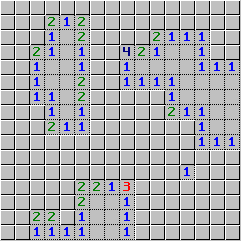
\includegraphics[width=0.5\textwidth]{slike/minolovec.png}
\podnaslov{Primer delno odprtega polja}
\end{slika}
\end{vprasanje}
\begin{odgovor}
\end{odgovor}
\end{naloga}
